\chapter{Spin wave theory of antiferromagnets}
\label{SpinWave}

In this Chapter we will study the magnon dispersion for the effective spin Hamiltonian obtained in the last two Chapters. The standard way of doing this is to use the Holstein-Primakoff transformation, which maps S-spin operators on a lattice to bosonic creation/annihilation operators. The linear approximation of this transformation leads to a bosonic Hamiltonian which can be diagonalized to obtain the magnon dispersion relation. Keeping higher order terms in this transformation is also useful to study scattering effects between magnons.

We will start studying the simplest model of spin interaction, the Heisenberg model. In the following sections we will add terms such as the DMI and the anisotropic NNN term derived in \ref{MKMHeff}.

\section{Heisenberg antiferromagnet}

We will start with the Heisenberg antiferromagnet:

\begin{equation}
\label{Heisenberg}
\hat{H} = J \sum_{\langle i j \rangle} \bs{S}_i \bs{S}_j
\end{equation}

In order to obtain the magnon Hamiltonian for this model we introduce the antiferromagnet Holstein-Primakoff transformation:

\begin{align}
S^+_{Ai} &= \sqrt{2S-\hat{a}^\dagger_i \hat{a}_i} \hat{a}_i \\
S^-_{Ai} &= \hat{a}^\dagger_i\sqrt{2S-\hat{a}^\dagger_i \hat{a}_i}  \\
S^z_{Ai} &= S - \hat{a}^\dagger_i \hat{a}_i \\
S^+_{Bj} &=\hat{b}^\dagger_j\sqrt{2S-\hat{b}^\dagger_j \hat{b}_j} \\
S^-_{Bj} &= \sqrt{2S-\hat{b}^\dagger_j \hat{b}_j} \hat{b}_j \\
S^z_{Bj} &= -S + \hat{b}^\dagger_j \hat{b}_j
\end{align}

Where $A$ and $B$ denote two Ne\'{e}l sublattices and $\hat{a}_i$, $\hat{b}_i$ are bosonic annihilation operators. In the large-S limit we approximate $ \sqrt{2S-\hat{a}^\dagger_i \hat{a}_i} \approx \sqrt{2S}$. Then, the exchange term becomes:

\begin{align*}
\bs{S}_i\bs{S}_j = S_i^zS_j^z + \frac{1}{2}\left(S_i^+S_j^- + S_i^-S_j^+ \right) = S \left( \hat{a}^\dagger_i \hat{a}_i + \hat{b}^\dagger_j \hat{b}_j + \hat{a}_i\hat{b}_j + \hat{a}^\dagger_i\hat{b}^\dagger_j \right) - \hat{a}^\dagger_i \hat{a}_i\hat{b}^\dagger_j \hat{b}_j - S^2
\end{align*}

Now the $S^2$ term is a constant that lowers the energy of the antiferromagnet, therefore is shall not be taken into account to compute the magnon dispersion. The term $\hat{a}^\dagger_i \hat{a}_i\hat{b}^\dagger_j \hat{b}_j$ is zeroth order in $S$ and therefore neglected. We can rewrite the sum over NN as:

\begin{equation}
\sum_{\langle i j \rangle} = 2\sum_{i \in A \delta}
\end{equation}

Where $\delta$ are the NN vectors. Using this, and the Fourier relations:

\begin{align}
\hat{a}_i^\dagger &= \frac{1}{\sqrt{N}} \sum_{\bs{k}} e^{i \bs{k} \cdot \bs{r}_i} \hat{a}_{\bs{k}}^\dagger \\
\hat{b}_j^\dagger &= \frac{1}{\sqrt{N}} \sum_{\bs{k}} e^{i \bs{k} \cdot \bs{r}_j} \hat{b}_{\bs{k}}^\dagger
\end{align}

Where the sum is over $\bs{k}$ in the first Brillouin zone. Using these relations, together with $\sum{i} e^{i(\bs{k}-\bs{k}')\cdot\bs{r}_i} = \delta_{\bs{k}, \bs{k}'}$ and denoting the number of sites by $N$ and the number of nearest neighbors by $z$, we find:

\begin{equation}
\hat{H} = -S^2JNz + 2JS \sum_{\bs{k} \bs{\delta}} \left( \hat{a}^\dagger_{\bs{k}}\hat{a}_{\bs{k}} + \hat{b}^\dagger_{\bs{k}}\hat{b}_{\bs{k}} + e^{i\bs{k}\bs{\delta}}\hat{a}_{\bs{k}}\hat{b}_{\bs{-k}} + e^{-i \bs{k}\cdot\bs{\delta}}  \hat{a}^\dagger_{\bs{k}}\hat{b}^\dagger_{-\bs{k}} \right)
\end{equation}

At this point it is common to define $\gamma_{\bs{k}} = \sum_\delta e^{i \bs{k} \cdot \bs{\delta}}$. Using $\bs{\delta}_1=\frac{a_0}{2}(1,\sqrt{3})$, $\bs{\delta}_2=\frac{a_0}{2}(1,-\sqrt{3})$, $\bs{\delta}_3=a_0(-1,0)$ (see Fig \ref{Fig.Magnon.Vecs}) and taking $a_0=1$, we can write this as:
\begin{equation}
\gamma_{\bs{k}} = 2e^{\frac{i}{2}k_x}\cos(\frac{\sqrt{3}}{2}k_y)+e^{-ik_x}
\end{equation}
Then denoting $z = \sum_\delta$ we get:

\begin{equation}
\label{MagnonicH}
\hat{H} = -S^2JNz + 2JS \sum_{\bs{k}} \left\{ z \left( \hat{a}^\dagger_{\bs{k}}\hat{a}_{\bs{k}} + \hat{b}^\dagger_{-\bs{k}}\hat{b}_{-\bs{k}} \right) + \gamma_{\bs{k}}\hat{a}_{\bs{k}}\hat{b}_{\bs{-k}} + \gamma_{-\bs{k}}\hat{a}^\dagger_{\bs{k}}\hat{b}^\dagger_{-\bs{k}} \right\}
\end{equation}

Which can be written in matrix form as:

\begin{equation}
\hat{H}_{\bs{k}} = 2JS\begin{pmatrix} 
z & \gamma_{\bs{k}} \\
\gamma_{-\bs{k}} & z
\end{pmatrix}
\end{equation}

Acting on the spinor $\Psi_{\bs{k}} = \left(\hat{a}_{\bs{k}},\hat{b}_{-\bs{k}}^\dagger \right)^T$. That is, $\hat{H} = -S^2JNz + \sum_{\bs{k}} \Psi_{\bs{k}} \hat{H}_{\bs{k}} \Psi^\dagger_{\bs{k}}$. In order to diagonalize this Hamiltonian we introduce the Bogoliubov transformation:

\begin{equation}
\label{Bogoliubov}
\begin{pmatrix}
\hat{\alpha}_{\bs{k}} \\
\hat{\beta}_{\bs{k}}
\end{pmatrix} = 
\begin{pmatrix}
u_{\bs{k}} & v_{\bs{k}}^* \\
v_{\bs{k}} & u_{\bs{k}}^*
\end{pmatrix}
\begin{pmatrix}
\hat{a}_{\bs{k}} \\
\hat{b}_{-\bs{k}}^\dagger
\end{pmatrix}
\end{equation}

Where $u_{\bs{k}}$ and $v_{\bs{k}}$ are complex functions satisfying $\abs{u_{\bs{k}}}^2-\abs{v_{\bs{k}}}^2 = 1$ in order to perserve the bosonic commutation relations. The inverse transformation is given by:

\begin{equation}
\label{BogoliubovInv}
\begin{pmatrix}
\hat{a}_{\bs{k}} \\
\hat{b}_{-\bs{k}}^\dagger
\end{pmatrix} = 
\begin{pmatrix}
u_{\bs{k}}^* & -v_{\bs{k}}^* \\
-v_{\bs{k}} & u_{\bs{k}}
\end{pmatrix}
\begin{pmatrix}
\hat{\alpha}_{\bs{k}} \\
\hat{\beta}_{\bs{k}}^\dagger
\end{pmatrix}
\end{equation}

Inserting this in \ref{MagnonicH} and ignoring constant terms we get:

\begin{align}
\hat{H} &= -S^2JNz + 2JS \sum_{\bs{k}} \left\{ \left( \hat{\alpha}_{\bs{k}}^\dagger \hat{\alpha}_{\bs{k}} +\hat{\beta}_{\bs{k}}^\dagger \hat{\beta}_{\bs{k}} \right) \left( z(\abs{u_{\bs{k}}}^2+\abs{v_{\bs{k}}}^2) -\gamma_{\bs{k}}u_{\bs{k}}^*v_{\bs{k}}^* - \gamma_{-\bs{k}}u_{\bs{k}}v_{\bs{k}} \right) + \right. \nonumber \\
&+ \hat{\alpha}^\dagger_{\bs{k}} \hat{\beta}^\dagger_{\bs{k}} \left( -2zu_{\bs{k}}v_{\bs{k}}^* + \gamma_{\bs{k}}(v_{\bs{k}}^*)^2+\gamma_{-\bs{k}}u_{\bs{k}}^2 \right) + \hat{\alpha}_{\bs{k}}\hat{\beta}_{\bs{k}} \left( -2zu_{\bs{k}}^*v_{\bs{k}} + \gamma_{\bs{k}}(u_{\bs{k}}^*)^2+\gamma_{-\bs{k}}v_{\bs{k}}^2 \right) + \nonumber \\
&\left. + \left( 2z\abs{v_{\bs{k}}}^2 - \gamma_{\bs{k}}u_{\bs{k}}^* v_{\bs{k}}^* - \gamma_{-\bs{k}}u_{\bs{k}}v_{\bs{k}} \right) \right\} \label{AfterBogo}
\end{align}

Therefore, in order to erase the non diagonal terms we impose:
\begin{equation}
\label{condition}
-2zu_{\bs{k}}v_{\bs{k}}^* + \gamma_{\bs{k}}(v_{\bs{k}}^*)^2+\gamma_{-\bs{k}}u_{\bs{k}}^2 = 0
\end{equation}
Notice that for the $\hat{\beta}_{\bs{k}}^\dagger\hat{\alpha}_{\bs{k}}$ term $-2zu_{\bs{k}}^*v_{\bs{k}} + \gamma_{\bs{k}}(u_{\bs{k}}^*)^2+\gamma_{-\bs{k}}v_{\bs{k}}^2=0$ is the same equation. This, together with $\abs{u_{\bs{k}}}^2-\abs{v_{\bs{k}}}^2 = 1$ determines $u_{\bs{k}}$ and $v_{\bs{k}}$. To see this, first notice that an overall phase in both $u_{\bs{k}}$ and $v_{\bs{k}}$ leads to the same physical state. We can use this fact to impose that $v_{\bs{k}}$ is real, and we can use $\abs{u_{\bs{k}}}^2-\abs{v_{\bs{k}}}^2 = 1$ to parametrize $u_{\bs{k}}$ and $v_{\bs{k}}$ in the following way:

\begin{align}
u_{\bs{k}} &= \cosh(\frac{\theta_{\bs{k}}}{2})e^{i \xi_{\bs{k}}} \label{Bogou} \\
v_{\bs{k}} &= \sinh(\frac{\theta_{\bs{k}}}{2}) \label{Bogov}
\end{align}

Where $\theta_{\bs{k}}$ and $\xi_{\bs{k}}$ are real functions to be determined. Introducing these relations in \ref{condition}:

\begin{equation}
- z\sinh(\theta_{\bs{k}}) +\gamma_{\bs{k}}e^{-i \xi_{\bs{k}}}\frac{ \cosh(\theta_{\bs{k}})-1}{2} +\gamma_{-\bs{k}}e^{i\xi_{\bs{k}}}\frac{ \cosh(\theta_{\bs{k}})+1}{2} = 0
\end{equation}

By taking $\xi_{\bs{k}}$ to be the phase of $\gamma_{\bs{k}}$, i.e. $\gamma_{\bs{k}} = \abs{\gamma_{\bs{k}}} e^{i\xi_{\bs{k}}}$ we get a real equation on $\theta_{\bs{k}}$. Altogether we find:

\begin{align}
\gamma_{\bs{k}} &= \abs{\gamma_{\bs{k}}} e^{i\xi_{\bs{k}}} \\
\tanh(\theta_{\bs{k}}) &= \frac{\abs{\gamma_{\bs{k}}}}{z}
\end{align}

This erases the non diagonal terms in \ref{AfterBogo} leading to a diagonal term:
\begin{equation}
z\cosh(\theta_{\bs{k}})-\abs{\gamma_{\bs{k}}}\sinh(\theta_{\bs{k}}) = \sqrt{z^2-\abs{\gamma_{\bs{k}}}^2}
\end{equation}

With this, we can rewrite \ref{AfterBogo} as:

\begin{align}
\hat{H} &= -S^2JNz + 2JS \sum_{\bs{k}}\left( \hat{\alpha}_{\bs{k}}^\dagger \hat{\alpha}_{\bs{k}} +\hat{\beta}_{\bs{k}}^\dagger \hat{\beta}_{\bs{k}}+1 \right)\epsilon_{\bs{k}}+2JS \sum_{\bs{k}}z(\abs{v_{\bs{k}}}^2-\abs{u_{\bs{k}}}^2) = \nonumber \\
&= E_0 + \sum_{\bs{k}}\left( \hat{\alpha}_{\bs{k}}^\dagger \hat{\alpha}_{\bs{k}} +\hat{\beta}_{\bs{k}}^\dagger \hat{\beta}_{\bs{k}} \right)
\end{align}

Where we used $\sum_{\bs{k}}=\frac{N}{2}$ and where $\epsilon_{\bs{k}} = 2JS \sqrt{z^2-\abs{\gamma_{\bs{k}}}^2}$. The ground state energy of this magnon Hamiltonian is:
\begin{equation}
E_0 = -JNz(S^2+S)+\sum_{\bs{k}}\epsilon_{\bs{k}} \label{HeisenbergMagnonGS}
\end{equation}
Note that the classical ground energy of \ref{Heisenberg} is $E_{cl}=-JNzS^2$, whereas the ground state that we obtained is lowered by:
\begin{equation}
\Delta E=-JNzS+\sum_{\bs{k}}\epsilon_{\bs{k}} = 2JS\sum_{\bs{k}}\left( \sqrt{z^2-\abs{\gamma_{\bs{k}}}^2} - z\right)
\end{equation}
Which is indeed negative since the terms in the sum are always negative. This term represents quantum corrections to the classical ground energy $E_{cl}$. Note that the fact that the quantum corrections lower the energy of the classical ground state means that the classical ground state (N\'eel order) is not an eigenstate of the Heisenberg Hamiltonian.

\section{Adding DMI}

Let's now consider

\begin{equation}
\hat{H} = J \sum_{\langle i j \rangle} \bs{S}_i \bs{S}_j + D \sum_{\langle \langle i j \rangle \rangle} \nu_{ij}\hat{e}_z \bs{S}_i \times \bs{S}_j
\end{equation}

The NNN DMI term will couple spins within the same sublattice. Using the HP transformation:

\begin{equation}
\hat{e}_z \bs{S}_i \times \bs{S}_j = \frac{i}{2}(S_i^+S_j^--S_i^-S_j^+) = \begin{cases}
             iS(\hat{a}_j^\dagger\hat{a}_i-\hat{a}_i^\dagger\hat{a}_j),  & \text{for } (i,j) \in A \\
             iS(\hat{b}_i^\dagger\hat{b}_j-\hat{b}_j^\dagger\hat{b}_i),  & \text{for } (i,j) \in B
       \end{cases} \quad
\end{equation}

Now we will make the sum over NNN in the following way:

\begin{equation}
\sum_{\langle \langle i j \rangle \rangle} = \sum_{i\in A \bs{\delta}^{NNN}} +  \sum_{i\in B \bs{\delta}^{NNN}}
\end{equation}

Where $\bs{\delta}^{NNN}$ are the NNN vectors (as depicted in Fig \ref{Fig.Magnon.Vecs}):
\begin{align*}
\bs{\delta}^{NNN}_1 &= \delta_1-\delta_3 = \frac{1}{2}(3, \sqrt{3}) \\
\bs{\delta}^{NNN}_2 &= \delta_2-\delta_1 = (0, -\sqrt{3}) \\
\bs{\delta}^{NNN}_3 &= \delta_3-\delta_2 = \frac{1}{2}(-3, \sqrt{3}) \\
\bs{\delta}^{NNN}_4 &= -\bs{\delta}^{NNN}_1 = -\frac{1}{2}(3, \sqrt{3}) \\
\bs{\delta}^{NNN}_5 &= -\bs{\delta}^{NNN}_2 = (0, \sqrt{3}) \\
\bs{\delta}^{NNN}_6 &= -\bs{\delta}^{NNN}_3 = \frac{1}{2}(3, -\sqrt{3}) \\
\end{align*}
\begin{figure}
\centering
  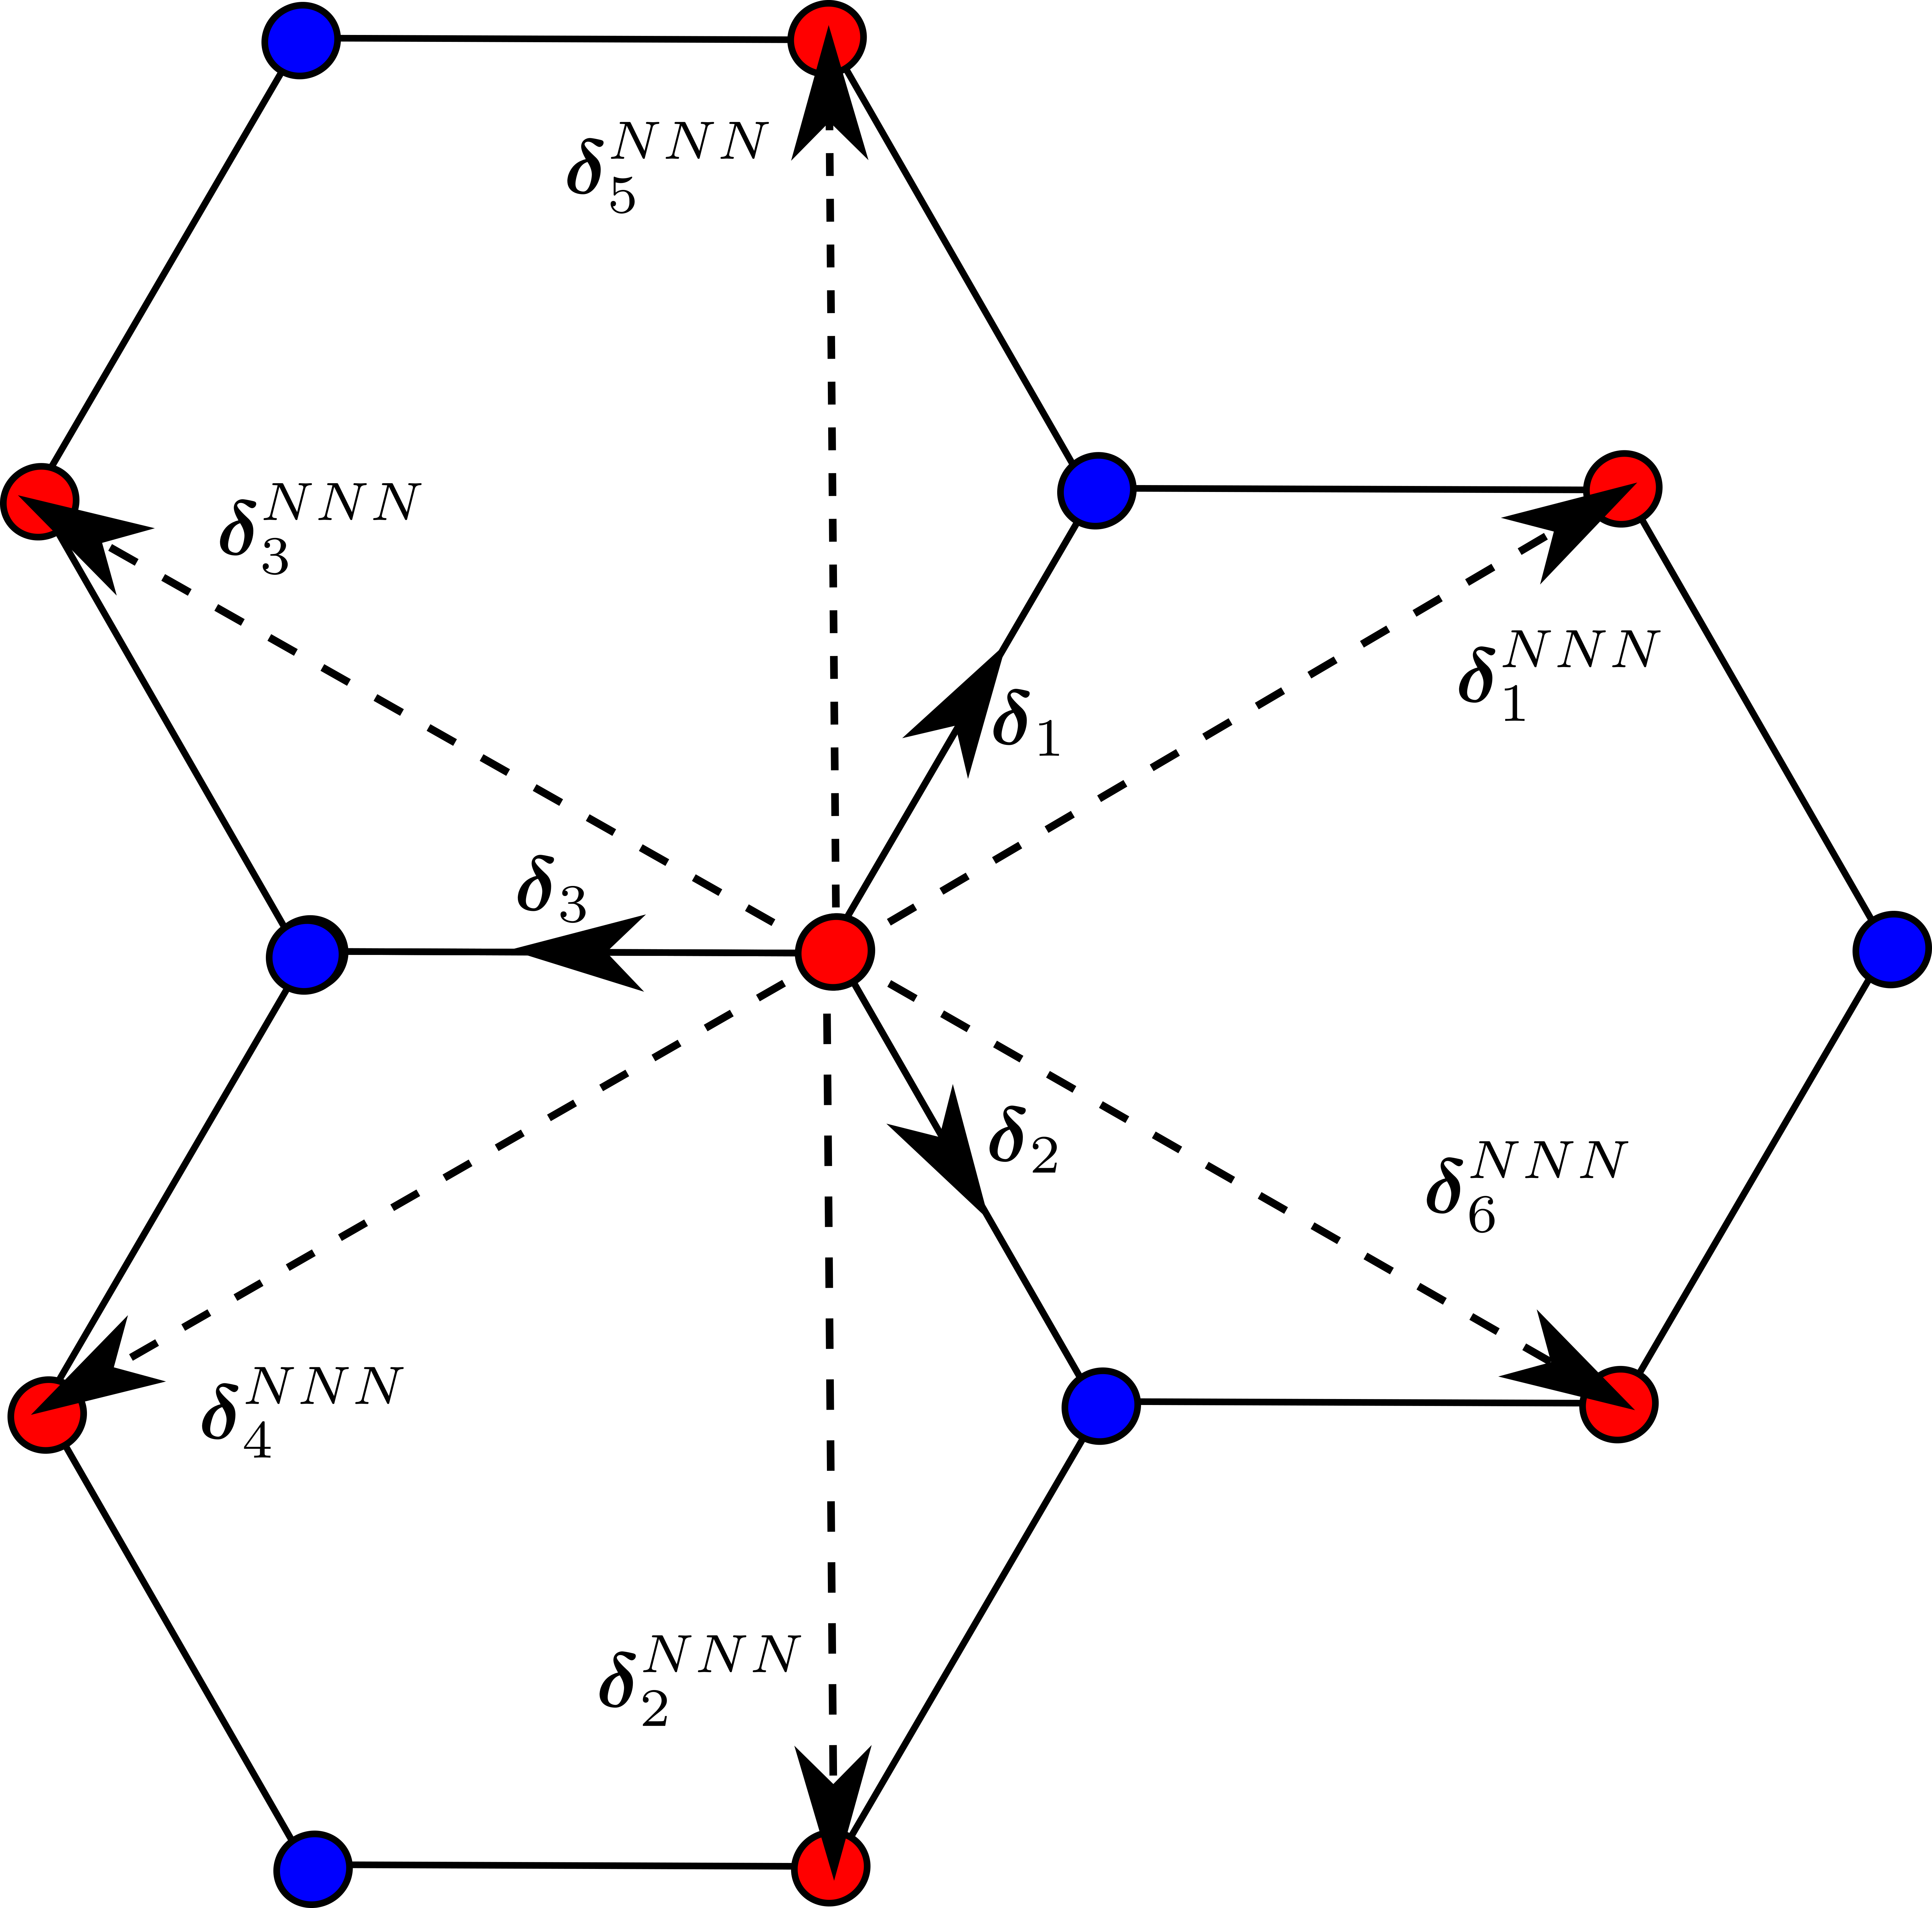
\includegraphics[width=0.7\linewidth]{../Figures/NNNvec.png}
  \caption{NN vectors $\bs{\delta}_a$ and NNN vectors $\bs{\delta}^{NNN}_a$. Red and blue denote sites of sublattices $A$ and $B$ respectively.}
\label{Fig.Magnon.Vecs}
\end{figure}
Notice that with these definitions, if $i$ is a site on the $A$ sublattice, $\nu_{i,i+\bs{\delta}^{NNN}_a}=+1$ for $a=1,2,3$ and $\nu_{i,i+\bs{\delta}^{NNN}_a}=-1$ for $a=4,5,6$. The opposite relations hold for $i$ in the $B$ sublattice.

 Following the same procedure as before we get and additional magnonic term:

\begin{equation}
D \sum_{\langle \langle i j \rangle \rangle} \nu_{ij}\hat{e}_z \bs{S}_i \times \bs{S}_j = 2JS\sum_{\bs{k}} \left\{ \Delta_{\bs{k}}\hat{a}^\dagger_{\bs{k}}\hat{a}_{\bs{k}} + \Delta_{-\bs{k}}\hat{b}^\dagger_{-\bs{k}}\hat{b}_{-\bs{k}} \right\}
\end{equation}

Where $\Delta_{\bs{k}} = \frac{Di}{2J}\sum_{\bs{\delta}^{NNN}} \nu_{i,i+\delta} (e^{i\bs{k}\cdot\bs{\delta}} -e^{-i\bs{k}\cdot\bs{\delta}})$, for $i$ in the $A$ sublattice. This can be rewritten as:
\begin{equation}
\Delta_{\bs{k}} = -\frac{2D}{J}\left\{ \sin(\bs{\delta}^{NNN}_1 \cdot \bs{k}) + \sin(\bs{\delta}^{NNN}_2 \cdot \bs{k}) + \sin(\bs{\delta}^{NNN}_3 \cdot \bs{k})\right\}
\end{equation}

Note that $\Delta_{\bs{k}}=-\Delta_{-\bs{k}}$ .The full magnonic Hamiltonian now is:

\begin{equation}
\label{MagnonicH2}
\hat{H} = -S^2JNz + 2JS \sum_{\bs{k}} \left\{ \hat{a}^\dagger_{\bs{k}}\hat{a}_{\bs{k}}(z+\Delta_{\bs{k}}) + \hat{b}^\dagger_{-\bs{k}}\hat{b}_{-\bs{k}}(z-\Delta_{\bs{k}}) + \gamma_{\bs{k}}\hat{a}_{\bs{k}}\hat{b}_{\bs{-k}} + \gamma_{-\bs{k}}\hat{a}^\dagger_{\bs{k}}\hat{b}^\dagger_{-\bs{k}} \right\}
\end{equation}

Or:

\begin{equation}
\hat{H}_{\bs{k}} = 2JS\begin{pmatrix} 
z + \Delta_{\bs{k}}& \gamma_{\bs{k}} \\
\gamma_{-\bs{k}} & z - \Delta_{\bs{k}}
\end{pmatrix} \label{MatrixMagnonDMI}
\end{equation}

In this case, applying the transformation \ref{Bogoliubov} leads to the same condition for the coefficients  $u_{\bs{k}}$ and $v_{\bs{k}}$, leading to:

\begin{align*}
\hat{H} &= -S^2JNz  + 2JS\sum_{\bs{k}} \left\{ \hat{\alpha}_{\bs{k}}^\dagger \hat{\alpha}_{\bs{k}} \left( \abs{u_{\bs{k}}}^2(z+\Delta_{\bs{k}}) + \abs{v_{\bs{k}}}^2(z-\Delta_{\bs{k}}) -\gamma_{\bs{k}}u_{\bs{k}}^*v_{\bs{k}}^*-\gamma_{-\bs{k}}u_{\bs{k}}v_{\bs{k}} \right) + \right. \\
&\left. + \hat{\beta}_{\bs{k}}^\dagger \hat{\beta}_{\bs{k}} \left( \abs{u_{\bs{k}}}^2(z-\Delta_{\bs{k}}) + \abs{v_{\bs{k}}}^2(z+\Delta_{\bs{k}}) -\gamma_{\bs{k}}u_{\bs{k}}^*v_{\bs{k}}^*-\gamma_{-\bs{k}}u_{\bs{k}}v_{\bs{k}} \right) + \right. \\
&\left. + \left( 2\abs{v_{\bs{k}}}^2 - \gamma_{\bs{k}}u_{\bs{k}}^*v_{\bs{k}}^*-\gamma_{-\bs{k}}u_{\bs{k}}v_{\bs{k}}\right) \right\}
\end{align*}

Where we already took \ref{Bogou} and \ref{Bogov}. The ground state energy $E_0$ remains the same as in the base Heisenberg model while the excitation modes $\hat{\alpha}_{\bs{k}}^\dagger$ and $\hat{\beta}_{\bs{k}}^\dagger$ change in the following way:

\begin{align}
\hat{H} &= E_0 + \sum_{\bs{k}} \left( \hat{\alpha}_{\bs{k}}^\dagger \hat{\alpha}_{\bs{k}} \epsilon_{\bs{k}}^+ +\hat{\beta}_{\bs{k}}^\dagger \hat{\beta}_{\bs{k}}  \epsilon_{\bs{k}}^- \right) \label{DispWithDMI} \\
\epsilon_{\bs{k}}^\pm &= 2JS \left( \pm \Delta_{\bs{k}} + \sqrt{z^2-\abs{\gamma_{\bs{k}}}^2} \right)
\end{align}

The new term $\pm \Delta_{\bs{k}}$ breaks the degeneracy between the $\alpha$ modes and the $\beta$ modes. In Figure \ref{Fig.Magnon.Disp} we plot the resulting energy dispersion of \ref{DispWithDMI}.

\begin{figure}
\centering
  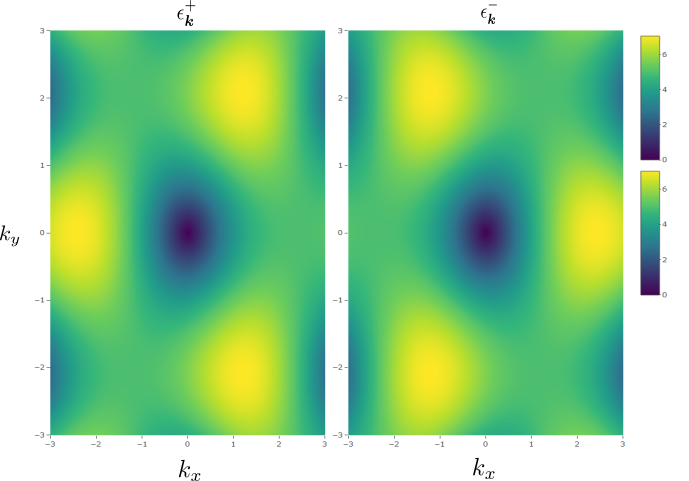
\includegraphics[width=0.7\linewidth]{../Figures/magnon_disp_2.png}
  \caption{The energy $\frac{\epsilon_{\bs{k}}^\pm}{JS}$ obtained for $D=0.1J$. For simplicity we take $E_0 = 0$. }
\label{Fig.Magnon.Disp}
\end{figure}

\section{NNN exchange}

We would like to see how the anisotropic spin interaction derived in \ref{MKMHeff} enters in the magnon Hamiltonian. To this end, we introduce now a term:

\begin{equation}
\sum_{\langle \langle i,j \rangle \rangle} \left\{ \Gamma_{xy}(S_i^xS_j^x + S_i^yS_j^y) + \Gamma_zS_i^zS_j^z\right\}
\end{equation}
Notice that taking $\Gamma_{xy} = -\abs{J_2}-\abs{\Gamma_2}$ and $\Gamma_z = -\abs{J_2}+\abs{\Gamma_2}$ describes the NNN exchange interaction and the NNN anisotropic interaction in \ref{MKMHeff}. In terms of bosonic operators we have:
\begin{equation}
\Gamma_{xy}(S_i^xS_j^x + S_i^yS_j^y) + \Gamma_zS_i^zS_j^z = \begin{cases}
             S\Gamma_{xy}(\hat{a}_i^\dagger\hat{a}_j+\hat{a}_j^\dagger\hat{a}_i) - S\Gamma_z(\hat{a}_i^\dagger\hat{a}_i+\hat{a}_j^\dagger\hat{a}_j),  & \text{for } (i,j) \in A \\
             S\Gamma_{xy}(\hat{b}_i^\dagger\hat{b}_j+\hat{b}_j^\dagger\hat{b}_i) - S\Gamma_z(\hat{b}_i^\dagger\hat{b}_i+\hat{b}_j^\dagger\hat{b}_j),  & \text{for } (i,j) \in B
       \end{cases} \quad
\end{equation}
Fourier transform leads to:

\begin{align*}
&\sum_{\langle \langle i,j \rangle \rangle} \left\{ \Gamma_{xy}(S_i^xS_j^x + S_i^yS_j^y) + \Gamma_zS_i^zS_j^z\right\}
= S\sum_{\bs{k}} (\Gamma_{xy}\Delta'_{\bs{k}}-4z\Gamma_z) (\hat{a}^\dagger_{\bs{k}}\hat{a}_{\bs{k}}+\hat{b}^\dagger_{-\bs{k}}\hat{b}_{-\bs{k}}) = \\
&=2JS\sum_{\bs{k}} \tilde{\Gamma}_{\bs{k}}(\hat{a}^\dagger_{\bs{k}}\hat{a}_{\bs{k}}+\hat{b}^\dagger_{-\bs{k}}\hat{b}_{-\bs{k}})
\end{align*}

Where we defined:
\begin{align*}
\Delta'_{\bs{k}} &= \sum_{\delta^{NNN}} \left( e^{i\bs{k}\cdot \bs{\delta}^{NNN}} +  e^{-i\bs{k}\cdot \bs{\delta}^{NNN}}\right) = 4\left\{ \cos(\delta^{NNN}_1\cdot\bs{k}) + \cos(\delta^{NNN}_2\cdot\bs{k}) + \cos(\delta^{NNN}_3\cdot\bs{k})\right\} \\
\tilde{\Gamma}_{\bs{k}} &= \frac{1}{2J}\left( \Gamma_{xy}\Delta'_{\bs{k}}-4z\Gamma_z \right)
\end{align*}
Therefore, now:

\begin{equation}
\hat{H}_{\bs{k}} = 2JS\begin{pmatrix} 
z + \Delta_{\bs{k}} + \tilde{\Gamma}_{\bs{k}} & \gamma_{\bs{k}} \\
\gamma_{-\bs{k}} & z - \Delta_{-\bs{k}} + \tilde{\Gamma}_{\bs{k}}
\end{pmatrix}
\end{equation}

This is the same as \ref{MatrixMagnonDMI} if we replace $z \rightarrow z + \tilde{\Gamma}_{\bs{k}}$, therefore the magnon Hamiltonian is:

\begin{align}
\hat{H} &= E_0 + \sum_{\bs{k}} \left( \hat{\alpha}_{\bs{k}}^\dagger \hat{\alpha}_{\bs{k}} \epsilon_{\bs{k}}^+ +\hat{\beta}_{\bs{k}}^\dagger \hat{\beta}_{\bs{k}}  \epsilon_{\bs{k}}^- \right) \\
\epsilon_{\bs{k}}^\pm &= 2JS \left( \pm \Delta_{\bs{k}} +  \sqrt{(z + \tilde{\Gamma}_{\bs{k}})^2-\abs{\gamma_{\bs{k}}}^2} \right)
\end{align}

This concludes our discussion of the magnons in the models derived in the last Chapter. The main difference of the magnonic Hamiltonian of a Kane-Mele system with a simple Heisenberg interaction is that the $\hat{\alpha}_{\bs{k}}^\dagger$ and $\hat{\beta}_{\bs{k}}^\dagger$ modes have non degenerate spectrum. This is arising from the addition of DMI in the model which breaks the symmetry of the system.

